\section{分子動力学シミュレーション}
\label{sec:md}
本研究では、大きく分けてモデリング、構造最適化、熱平衡化、サンプリング、解析の5つのステップを経た。

\subsection{モデリング}
モデリングでは、欠損部位の補完、結晶水の同定、膜タンパク質の構造準備の3つのステップを経た。

\subsubsection{欠損部位の補完}
PDBに登録されている膜タンパク質の構造データは、全ての残基位置が定まっているわけではない。なぜならX線結晶構造解析において、揺らぎが大きい部位は見えないからである。
$\beta_2$ARでは、プログラムMODELER\cite{Sali1995}を用いて細胞内ループ3(ICL3)、N末端、C末端の欠損部位を補完した。
MODELERではホモロジーモデリングを利用して、既存のPDBデータから欠損部位の座標を予測する。

\subsubsection{結晶水の同定}

膜タンパク質内の結晶水が重要な役割を果たしていることから、タンパク質内部の結晶水の存在場所を推定するプログラム DOWSER\cite{Zhang1996}を用いてエネルギー的に安定な水分子を同定し、構造に含める作業を行った。
DOWSERはエネルギー的に安定な水分子の位置を計算し、これを構造データに追加することが可能である。この手順により、機能的に重要な膜タンパク質の構造を構築した。

\subsubsection{膜タンパク質の構造準備}
初めに、膜タンパク質と脂質膜の複合体構造は、モデリングツール CHARMM-GUI\cite{CHARMMGUI}を用いて作成した。
複合体構築には置換法(Replacement Method)を採用し、タンパク質を囲むように脂質二重膜を配置した。
以下にCHARMM-GUIの設定手順を示す。
\begin{enumerate}
    \item \textbf{初期設定}: CHARMM-GUIサイトで\textit{Protein/Membrane System}を選択し、準備したPDBファイルをアップロード。
    \item \textbf{分子選択}: リガンドと結晶水を含めるように選択。
    \item \textbf{プロトン化とジスルフィド結合の設定}: プロトン化残基やジスルフィド結合を指定。
    \item \textbf{脂質二重膜の構築}: \textit{Heterogeneous Lipid}を選択し、脂質のXY軸長を80~\AA\ $\times$ 80~\AA\ に設定。
    \item \textbf{イオン追加}: NaCl濃度を0.15Mに設定し、Na$^{+}$ と Cl$^{-}$を追加。
\end{enumerate}
分子動力学計算はAmber力場で行うため、CHARMM-GUIで出力されたpdbファイルをAmber形式に変換する。

続いて、リガンドの力場構築には、AmberToolsの\texttt{antechamber}と\texttt{parmchk2}ツールを使用した。

続いて、実際にシミュレーションを行うシステムに対して、プロトン化状態の修正、ジスルフィド結合の形成を行う。
プロトン化状態の修正に関しては、タンパク質構造が与えられた環境下で適切なプロトン化状態を取るように、残基の名前を変更する必要がある。
本研究では、脂質環境下にあるGlu122はプロトン化したグルタミン酸(GLHモデル)として扱った。
膜表面側にある残りのGlu,Asp,Arg,Lysは中性(pH=7)での状態を採用した。
%GLu122
%https://pubs.acs.org/doi/full/10.1021/jp506579a
最後に、タンパク質-リガンド複合体の分子動力学シミュレーションで用いるためのシミュレーション用のファイルを準備した。
シミュレーションに使用する力場関数に関して、
タンパク質にはff12SB、
脂質にはlipid21、
リガンドにはgaff2、
水分子にはtip3pモデルを用いた。

系のユニットセルサイズはCHARMM-GUIで得られた情報に基づいて、以下のように指定する。
\begin{table}[!ht]
  \centering
  \caption{シミュレーションに用いた系の大きさ}
  \resizebox{\textwidth}{!}{
      \begin{tabular}{lll}
          \hline
          モデル名          & 原子数  & ボックスの大きさ (x, y, z) \\
          \hline
          inactive (3P0G)  & 84225 & (80.2377, 80.2377, 113.064) \\ 
          active (2RH1)    & 70608 & (80.0239, 80.0239, 136.043) \\ 
      \end{tabular}
  }
  \label{tab:system_size}
\end{table}


\subsection{構造最適化}
構造最適化は3つのステップに分けて行った。
全てのステップにおいて、最急降下法で最小化を開始し、200ステップ後に共役勾配法(CG法)へ切り替えている。
初めに、水素以外の全ての原子に位置制約を課し、タンパク質周辺の脂質や水分子の構造最適化を行った。
続いて、膜タンパク質の主鎖原子、リガンドの重原子、脂質のhead部分に位置制約を課し、膜タンパク質の側鎖原子や水分子の構造最適化を行った。
最後に、上記の束縛力を弱めて、全体の構造を最適化した。

\subsection{熱平衡化}
熱平衡化は4つのステップに分けて行った。
初めに、NVTアンサンブルで系を徐々に加熱させた。
初期速度は温度$T = 0 \rm{[K]}$のマクスウェル分布に従って与え、 
100 $\rm{ps}$で温度を$T = 310 \rm{[K]}$まで上昇させた。
タンパク質とリガンドに対して$2.0 \, \text{kcal/mol/\AA}^2$の拘束を加えた。

続いて、NVT条件下で200 $\rm{ps}$のシミュレーションを行った。
Langevin法を用いた温度制御を行いながら、$T = 310 \rm{[K]}$で設定した。
タンパク質とリガンドの位置拘束の重みを$0.1 \, \text{kcal/mol/\AA}^2$に設定した。

続いて、上記と同様のNVT条件下で、今度は位置拘束を全て外して、200 $\rm{ps}$のシミュレーションを行った。

最後に、NP\gamma T条件下で700 $\rm{ps}$のシミュレーションを行った。
Langevin法を用いた温度制御とBerendsen法を用いた圧力制御を行いながら、$T = 310 \rm{[K]}$で設定した。
位置拘束を外し、膜系のシミュレーション用に表面張力\gamma = 17 \, \text{dyne/cm}で設定した。

\subsection{サンプリング}
ここではNP\gamma Tシミュレーションによるサンプリングを56 $\rm{ns}$行った。
設定は、熱平衡化で行ったNP\gamma Tシミュレーションと同様である.

\subsection{保存された結晶水の同定}
保存された結晶水を同定するために、サンプリングで得られたシミュレーションデータから水分子の位置とその密度を分析した。
具体的には、シミュレーションの各タイムステップで得られる水分子の座標を一辺50\,\text{\AA}の格子状に集約し、サンプリングで得られたトラジェクトリの半分以上で保存されている水分子を同定した。

\subsection{NVE}
最後にNVEシミュレーションによるサンプリングを行った。
初期状態として、NP\gamma Tシミュレーションによるサンプリングで得られた座標と速度を用いた。
保存した座標と速度から\Delta t = 0.5 fs、1000 $\rm{ps}$のシミュレーションを実行した。
最終的に、inactive状態active状態双方で1000psトラジェクトリを計10本取得した。
その後、分子動力学(MD)シミュレーションを用いて得られた、
inactive状態とactive状態におけるNVEトラジェクトリーの全フレームの座標を時間平均することで得られる平均構造を取得した。

\section{グラフ理論}
\label{sec:graph theory}

\subsection{ネットワーク構築}

本研究では、ノードをアミノ酸残基とし、以下の条件に基づいてエッジを形成した。
\begin{itemize}
    \item \textbf{隣接する残基間のエッジは削除する}  
    本研究ではinactive状態からactive状態へのネットワークの再編に着目しているため、フォールディングの過程で存在し続けている隣接残基間の共有結合は取り入れずに、構造安定性や機能に関連する残基間相互作用であるnative contactのみに焦点を当てる。
    \item \textbf{残基ペア間の最短距離が3\,\text{\AA}未満である場合、エッジを形成する}  
    \item \textbf{エッジの重みは、残基間最短距離の2乗逆数の平均$\langle \frac{1}{d^2} \rangle$を用いる}  
    inactive状態とactive状態におけるトラジェクトリの平均構造から、残基間最短距離の2乗逆数の平均$\langle \frac{1}{d^2} \rangle$を得る。熱揺らぎなど分子の動的な挙動の性質を反映している平均構造を用いることで、タンパク質の実際の挙動をより忠実に表現する。    
  \end{itemize}

エネルギー輸送経路はアロステリックな情報伝達経路と関係しているという仮説の下で計算された$\beta_2$ARのエネルギー輸送経路の研究において、
$\beta_2$ARはリガンドとの非共有結合(極性・非極性相互作用)を介したエネルギー輸送が主であったことがわかっている\cite{Helmer2022}。


また、構造、局所的ダイナミクス、相互作用を反映する物理的変数である残基間熱流の自己相関関数に基づく残基間局所熱伝導率の値を決定する上で
「残基間の最短距離の2乗逆数の平均」と「最短距離の分散の2乗逆数の平均」が支配的な役割を果たすことが、
HP36(pdb code:1vii)のrandom forest解析によりわかっている\cite{Wang2024}。
%randomforest
%https://pubs.acs.org/doi/full/10.1021/acs.jpcb.4c03475?casa_token=kIrJZ9z3XmoAAAAA%3AdCe19514PuUO6o1nBQVelnZulU8CeElXxLuO5_ugsWtic1wHX1ucufyBTAiRsAKwQ-9gSQxdEWGIOJI

この解析を、残基数110のPDZ3(pdb code:1tq3)という、残基数36のHP36よりも残基数の多いタンパク質に適用したのが、以下の図である。

\begin{figure}[htbp]
    \centering
    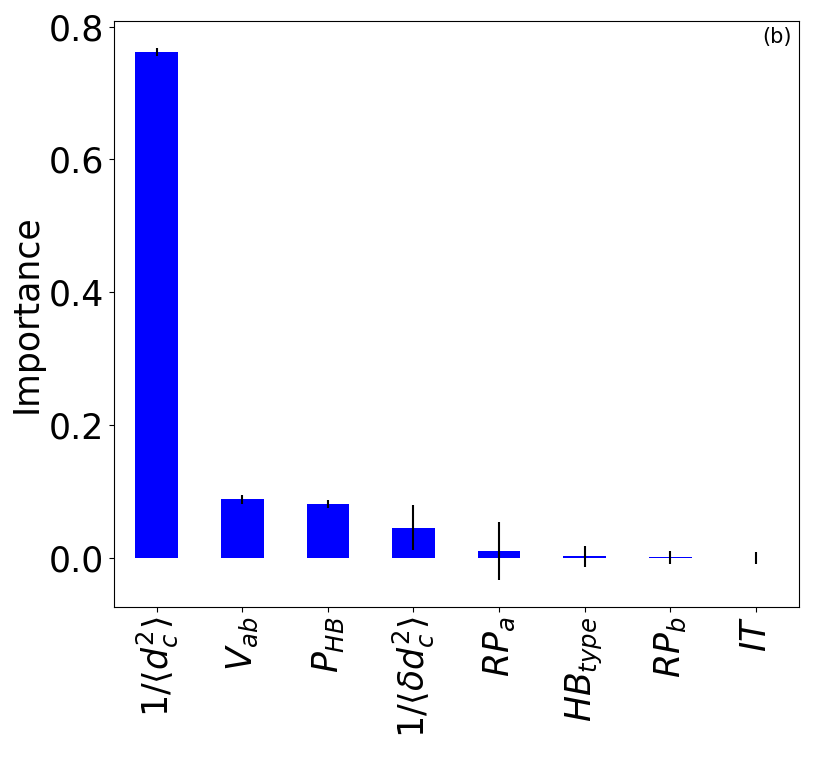
\includegraphics[width=1.0\textwidth]{random-forest_permutation_importance.png}
    \caption{PDZ3において、平均最短距離⟨dc⟩がそれぞれ4Å未満の残基ペアに対する、残基間局所熱伝導率の変数重要度のVIPスコアプロット。}
    \label{fig:random_forest}
\end{figure}

\newpage

PDZ3になると残基間の「最短距離の2乗逆数の平均」が有意に局所熱伝導度に影響していることがわかる。

この文献で用いられているHP36、PDZ3、本研究で用いる$\beta_2$ARのinactive/active構造の
残基ペア間の最短距離が3\,\text{\AA}未満のエッジ数の中で、hydrophobic相互作用を形成する残基ペアが占める割合を比較すると、
$\beta_2$ARではhydrophobic相互作用を形成する残基ペアの割合がPDZ3よりも増加する。

\begin{table}[!ht]
    \centering
    \caption{タンパク質のノード数と、残基ペア間の最短距離が3\,\text{\AA}未満のエッジ数の中でhydrophobic相互作用を形成する残基ペアが占める割合}
    \resizebox{\textwidth}{!}{
    \begin{tabular}{p{2cm}ccc}
        \hline
        モデル名                            &  ノード数  &  3\,\text{\AA}未満の疎水残基率\\
        \hline 
        HP36                               &  36  &  66.14\%  \\ 
        PDZ3                               &  110  &  72.19\%  \\ 
        $\beta_2$AR(inactive)              &  350  &  75.32\%  \\ 
        $\beta_2$AR(active)                &  349  &  75.77\%  \\ 
    \end{tabular}
    }
    \label{tab:hydrophobic_rate}
  \end{table}


このことから、$\beta_2$ARの3\,\text{\AA}未満のエッジにおいても、
残基ペア間の最短距離が残基間の挙動を反映する支配的な変数であると言える。

そこで本研究では、残基ペア間の最短距離が3\,\text{\AA}未満のエッジにおいて、
残基間最短距離の2乗逆数の平均$\langle \frac{1}{d^2} \rangle$をエッジの重みとする静的ネットワークを構築する。


\subsection{Louvain法によるコミュニティ検出}

Louvain法は、ネットワークにおけるコミュニティ構造を検出するための効率的なアルゴリズムである。
本研究では、Louvain法\cite{Blondel2008}を実装してネットワークデータを解析し、最適なコミュニティ分割とモジュラリティの評価を行った。
%louvain方の引用2008
%https://iopscience.iop.org/article/10.1088/1742-5468/2008/10/P10008/meta?casa_token=gUnIfMpEgFUAAAAA:CzncxXVCSbFF0gBux5xGhAWMnQDOio3eBOyMY8VDngPf7-LFexsnOz5gan6uHE0dlL7JrLJQAdwuwauUSrrCsmDHg0g
\subsubsection{モジュラリティの定義}
モジュラリティ$Q$は、ネットワーク内で検出されたコミュニティ構造の質を評価する尺度である。
具体的には、同一コミュニティ内に存在するエッジの密度が、ランダムに生成されたネットワークと比較してどれだけ顕著に密集しているかを示す。
モジュラリティは次式で定義される:
\begin{equation}
Q = \sum_{c \in \text{コミュニティ}} \left( \frac{m_c}{m} - \left( \frac{K_c}{2m} \right)^2 \right),
\end{equation}
ここで、$m_c$はコミュニティ$c$内のエッジの重み合計、$m$はネットワーク全体のエッジの重み合計、$K_c$はコミュニティ$c$内のノードの次数の合計である。
この定義により、同一コミュニティ内でのエッジ密度が高い場合にモジュラリティの値が大きくなり、ネットワークのコミュニティ構造がより明確であることを示す。

\subsubsection{アルゴリズムの流れ}
Louvain法は以下の2つのステップを繰り返してコミュニティを検出する:
\begin{enumerate}
    \item \textbf{局所移動ステップ:} 各ノードを隣接するコミュニティに移動させ、モジュラリティの増加が最大となる配置を探索する。
    このプロセスにおいて、モジュラリティの変化量$\Delta Q$は以下で計算される:
    \begin{equation}
    \Delta Q = \Delta Q_{\text{削除}} + \Delta Q_{\text{挿入}},
    \end{equation}
    ここで、$\Delta Q_{\text{削除}}$はノードを元のコミュニティから削除した際のモジュラリティの変化量、$\Delta Q_{\text{挿入}}$はノードを新たなコミュニティに追加した際のモジュラリティの変化量である。
    \item \textbf{集約ステップ:} 検出されたコミュニティを1つのノードとして扱い、新しいネットワークを構築する。この操作を通じて、階層的なコミュニティ構造を得ることが可能である。
\end{enumerate}

本研究では、Pythonを用いてLouvain法を実装した。
モジュラリティの増加が小さい場合に収束するよう、収束条件として閾値$\epsilon = 10^{-7}$を設定した。
また、ノードの移動においてランダム性を導入し、複数回の試行によりモジュラリティの最適解を探索した。
そして、100回の試行の中で最大のモジュラリティおよびその標準偏差と標準誤差を算出した。